\documentclass{article}
\usepackage{../../Self_Style}

\title{Phys 20AL Week 10 Lab Report: Lense and Mirrors}
\author{Zih-Yu Hsieh}
\date{\today}

\begin{document}
\maketitle

\tableofcontents

\hfil

\section{Introduction}
For different lenses / mirrors, there are different effects on refracting the light: For instance, convex lenses (or lenses with positive focal length) and concave mirrors would concentrate the light, while concave lenses (or lenses with negative focal length) would separate the light to wider ranges in contrast to that.

For these lenses, a simple way of characterizing them is the radius of curvature $r$, and the focal length $f=\frac{r}{2}$ (on the limit of small angles, the focal length mathematically is approximately this value). 

The aim for this lab is to understand the relation between the distance of the lens / mirror from the object, the focal length, and the image. Which, the first part of the experimetn is designed to measure the focal length, the second part is proposed for lens equation $\frac{1}{s_o}+\frac{1}{s_i}=\frac{1}{f}$,  the third part is then verify the transversal magnification for provided lens, and the fourth part is for explaning the mirage setup in the lab.

\newpage

\section{Experimental Setup}
The lab equipments include: A light source (with multiple mode: including point light source and parallel light source), a track with length provided (to simplify the distance measurement, by reading the values on the track), several lenses (including 3 convex lenses, 1 concave lens, and 1 concave mirror), a bourd (for convex lenses' images), and a half-transparent paper (for concave lens / mirror's image).

The setup is simple: fix the light source on one end of the track, and set the lenses / mirror on the track (at the desired position), then use the board / the paper to observe the position of the image.

\begin{figure}[h!]
    \centering
    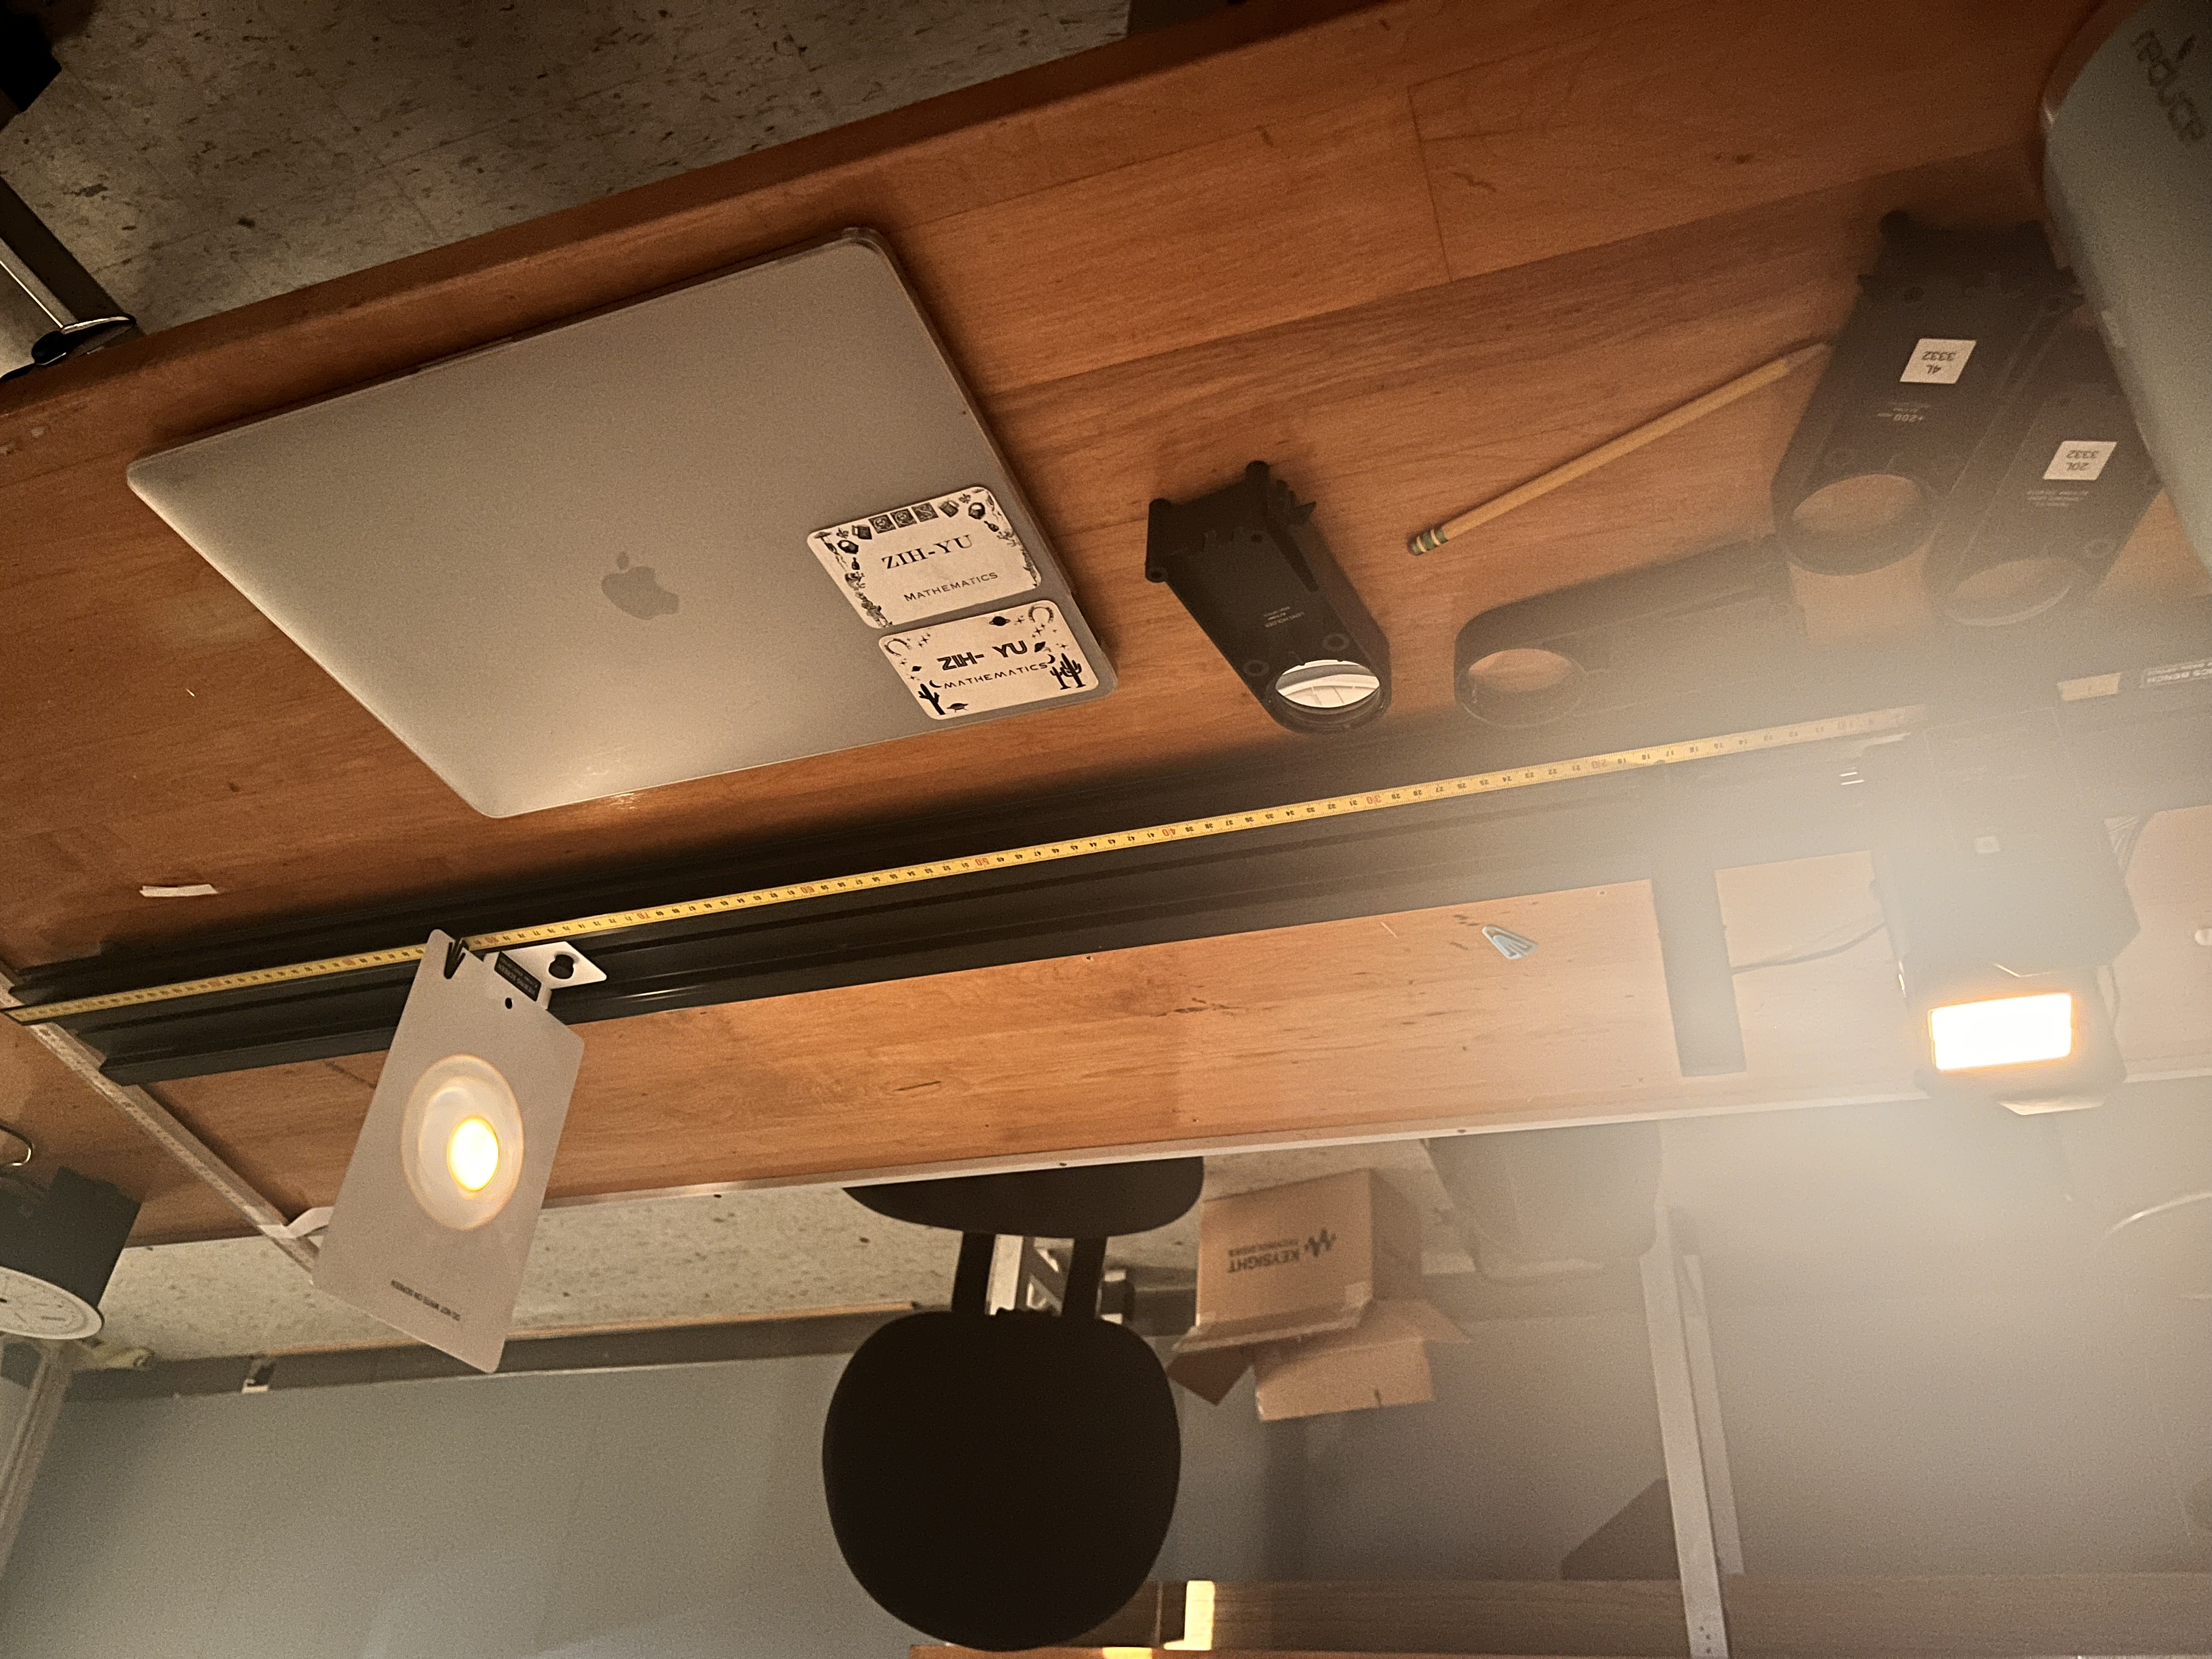
\includegraphics[width=100mm]{lab_setup10.png}
    \caption{Picture of the actual Lab Setup}
    \label{fig:lab_setup}
\end{figure}

\hfil

For the Mirage setup, it includes two concave mirrors with the same focal length (one has a hole at the centor) (the focal length is specifically designed to be twice as the height of the mirror), together with a small object.

Th two mirrors are stacked together with the mirror sides facing each other (the one has a hole is on top), then placed the small object at the center of the bottom mirror, which is observable through the hole of the top mirror.

\begin{figure}[h!]
    \centering
    \begin{subfigure}[t]{0.4\textwidth}
        \centering
        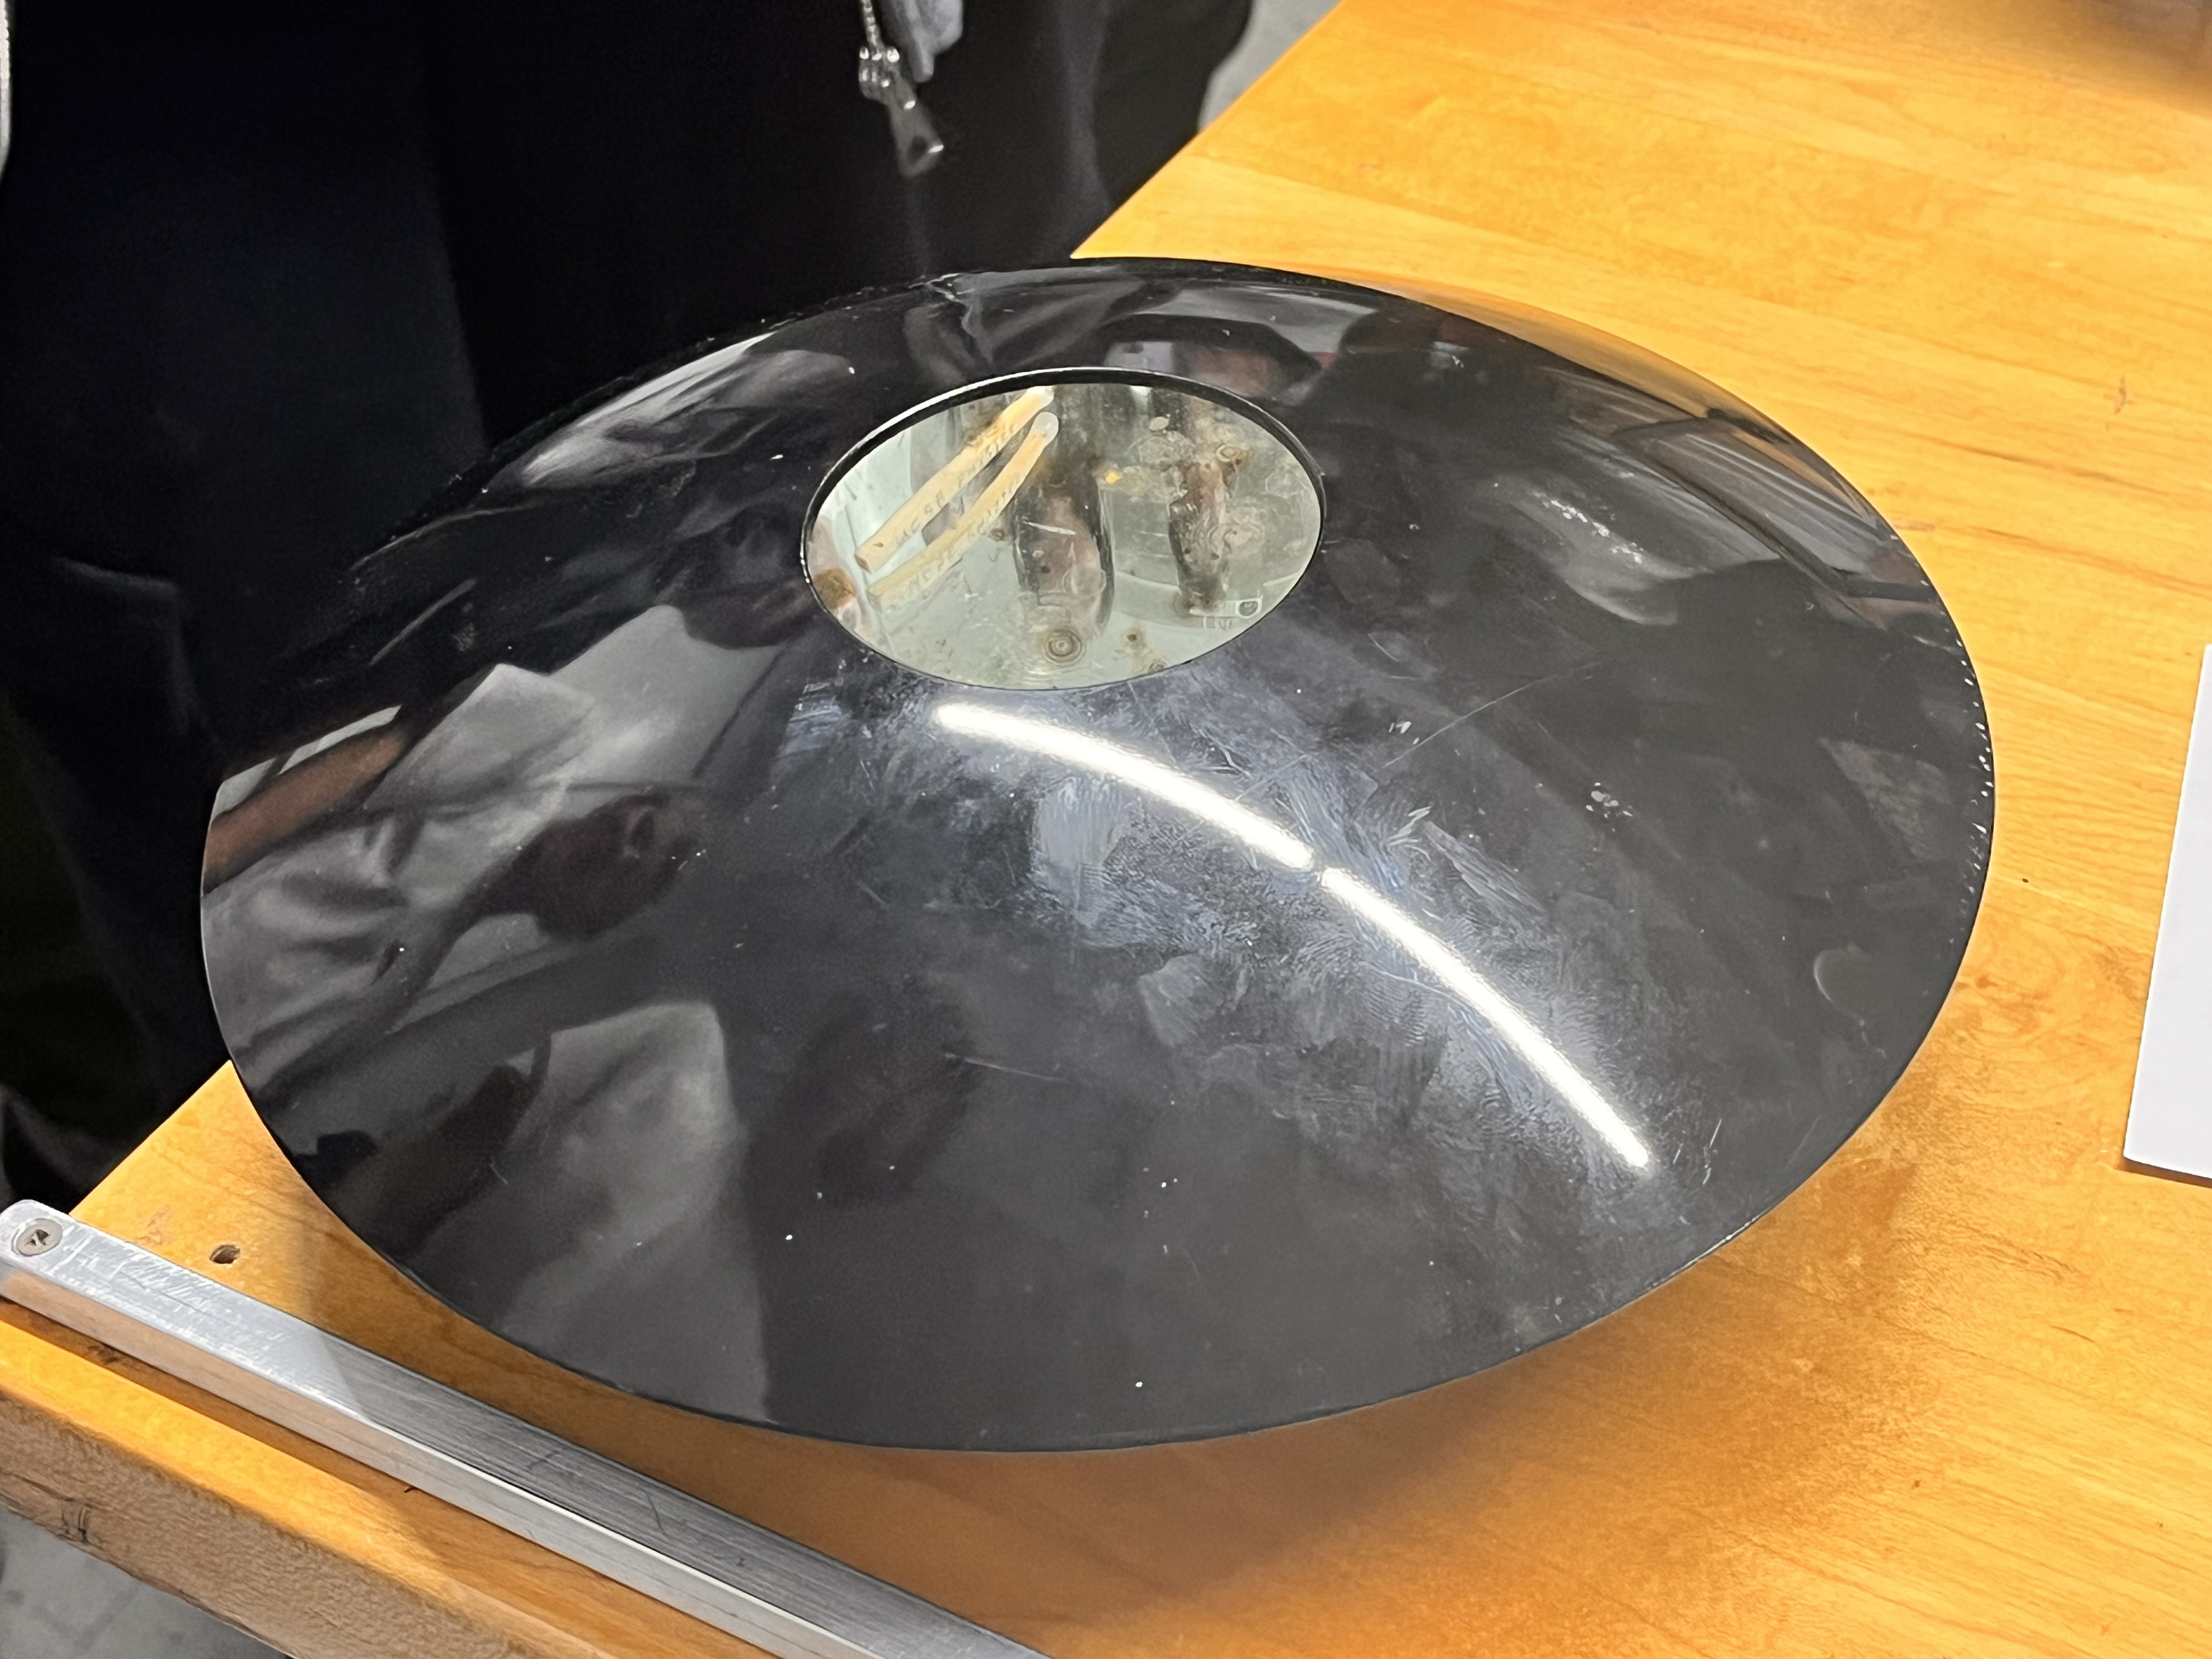
\includegraphics[width=\linewidth]{mirage.png}
        \caption{Photo of the Mirage Setup}
        \label{fig:mirage_setup}
    \end{subfigure}
    \hfil 
    \begin{subfigure}[t]{0.4\textwidth}
        \centering
        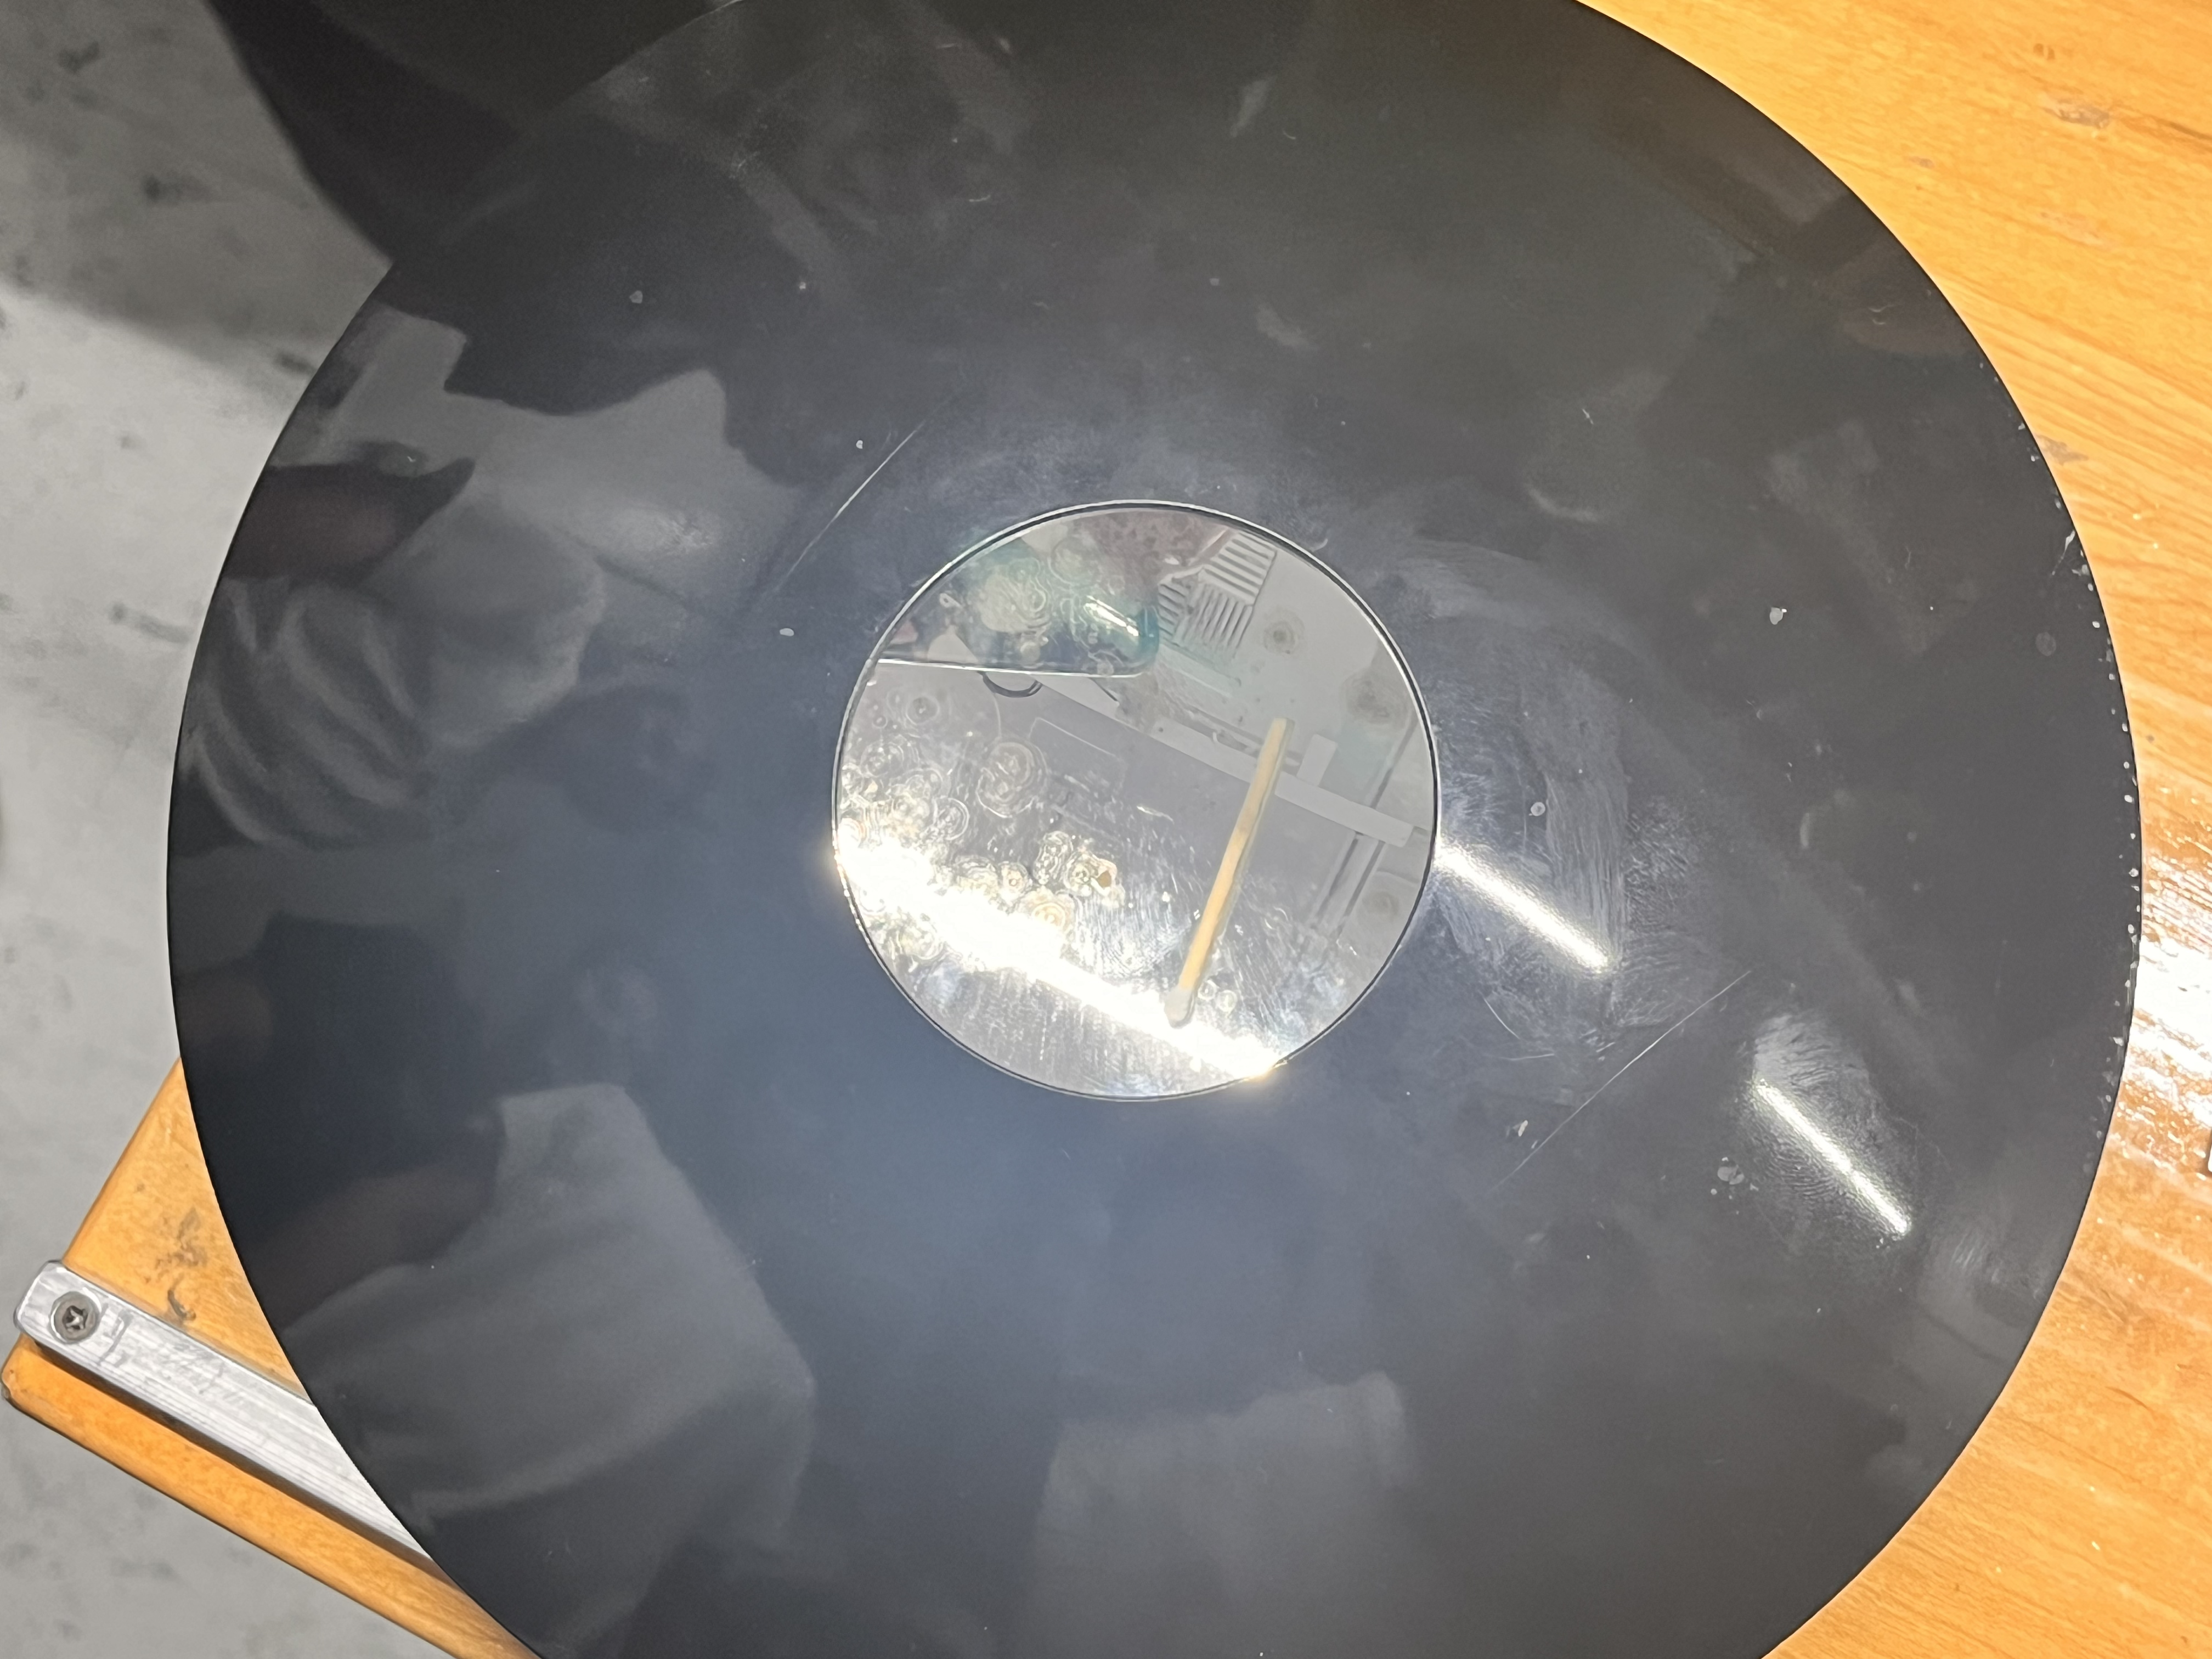
\includegraphics[width=\linewidth]{mirage_top.png}
        \caption{Top Photo of the Mirage Setup}
        \label{fig:mirage_setup_top}
    \end{subfigure}
\end{figure}

\newpage

\section{Methods of Measurement and Quantities to Measure}
There are three sections to consider:

\subsection{Focal Length Measurement}
This section of the lab will measure the focal length of the lenses and the mirrors (unit: mm). For each lens / mirror, one will measure a total of 3 trials, and take the average focal length.

For the three convex lenses, since in theory a point light source on the focal point (with light radiating outward from the source) becomes parallel light after passing through the lense, the distance of the point light source away from the lense that generates such phenomenon will be recorded as the focal length.

For the concave mirror, one will use a parallel light source, and use a half-transparent paper to find the position where the reflected light focuses on (in between the mirror and the light source). (\textbf{Rmk}: The half-transparent paper is used to ensure the light source is not fully blocked, so it's still possible to observe the focal point without blocking all light sources).

For the concave lens, one will use a parallel light source with multiple slits, measure the gaps distance between the slits when project onto the board under different board positions, then derive the focal length using some equations. Which, the distance of the board away from the concave lens include $100, 200,$ and $300$ mm.

\hfil

\subsection{Lense Equation:}
This section of the lab will verify the lense equation: Let $s_o$ denotes the distance between the light source and the lens, while $s_i$ denotes the distance between the image and the lens, and $f$ denotes the focal length, the equation states $\frac{1}{s_o}+\frac{1}{s_i}=\frac{1}{f}$ (with the position in front of the lens be negative, and the position behind the lens be positive).

Here, it measures two convex lenses and one concave lens. For each lens, $5$ different source distance $s_o$ will be tested (dependent on the lens), both $s_o$ and $s_i$ will be measured using the track's distance labels, and the focal length $f$ will be deduced from the data gathered in the First Section (which measured the focal length of each lens).

Also, the position of the image will be determined as follow:
\begin{itemize}
    \item For convex lenses, the image will be projected onto the board, and by adjusting the position of the board tiill the image is clear / focused, that determines the image position.
    \item For concave lenses, the half-transparent board will again be inserted in between the light source and the lense to measure where the light focuses at to determine the image position.
\end{itemize}

\hfil

\subsection{Transversal Magnification}
For this section, with light source distance $s_o$ and image distance $s_i$, the transversal magnification $M_T := -\frac{s_i}{s_o}$. This is determined for one convex and one concave lens, together with $5$ different light source distance $s_o$.

The data for this section will be derived from the data collected for the Lense Equation Section.

\newpage

\section{Experimental Procedure}
\subsection{Focal Length Measurement}
The following procedure will be performed for convex lenses:
\begin{enumerate}
    \item Turn the light source to a point light source, and set the lens / mirror in the middle of the track.
    \item Insert the board behind the lens to observe the radius of the light after passing through the lens, and move the board to various distances away from the lens to observe the change of radius.
    \item Adjust the position of the lens away from the light source, until the radius mentioned in Step 2 no longer changes when adjusting the board position. Record the distance between the light source and the lens as the focal length.
    \item Repeat Step 3 for a total of three times.
    \item Repeat Step 3 and 4 for different convex lenses.

\end{enumerate}

\hfil

Now, the following procedure will be performed for the concave mirror:
\begin{enumerate}
    \item Turn the light source to a parrallel light source, and set the lens / mirror in the middle of the track.
    \item Insert the half-transparent paper in between the source and the mirror, and move the paper until observing focused light dot on the paper. Record the distance of the paper away from the mirror as th focal length.
    \item Repeat Step 3 for a total of three times.
\end{enumerate}

\hfil

Finally, the following procedure will be performed for the concave lens:
\begin{enumerate}
    \item Turn the light source to a parallel light source with slits, and insert the board near the end of the track.
    \item Record the gaps between the consecutive light patterns that occur on the boad.
    \item Insert the lens in the middle of the track.
    \item Adjust the board to some distance away from the lens, and measure the gaps between the light patterns on the board. Record both the distance of the board, and the gaps length.
    \item Repeat Step 4 for different board positions.
\end{enumerate}

\newpage

\subsection{Lense Equation and Transversal Magnification}
The following procedure will be performed for convex lenses:
\begin{itemize}
    \item Turn the light source to parallel light source, and set the lens with a desired distance $s_o$ away from the light source.
    \item Insert the board behind the lens, adjust its position until the light source is focused at a point on the board. Record this board distance away from the lens as the image distance $s_i$.
    \item Repeat Step 1 and 2 for all the desired light source distance $s_o$.
\end{itemize}

\hfil

The following procedure will be performed for concavee lenses:
\begin{itemize}
    \item Turn the light source to point light source, and set the lens with a desired distance $s_o$ away from the light source.
    \item Insert the half-transparent paper in between the light source and the lens, and find the point where the light focuses on the paper. Record this as the image distance $s_i$.
    \item Repeat Step 1 and 2 for all desired light source distance $s_o$.
\end{itemize}

\hfil

\section{Experimental Data and Data Analysis}
\subsection{Focal Length Measurement}
For convex lenses, one has the following focal lengths measurement:
\begin{table}[h!]
\centering
\begin{tabular}{l||ccc|cc}
\hline
\diagbox[width=4cm,height=1cm]{\textbf{Convex Lenses}}{\textbf{Trial}} & \textbf{1} & \textbf{2} & \textbf{3} & \textbf{Ave (mm)} & \textbf{SD (mm)} \\
\hline
Lens 1 & 81.000 & 82.500 & 80.000 & 81.750 & 1.258 \\
Lens 2 & 160.000 & 162.000 & 163.000 & 161.000 & 1.528 \\
Lens 3 & 204.000 & 202.000 & 203.500 & 203.000 & 1.041 \\
\hline
\end{tabular}s
\caption{Focal Lengths for Convex Lenses (unit: mm)}
\label{tab:convex_focal}
\end{table}

Which, in comparison to the average focal length, the standard deviation in each case is small, which can treat the averages as the representatives of focal lengths.

\hfil

For concave mirror, one has the following focal lengths measurement:
\begin{table}[h!]
\centering
\begin{tabular}{l||ccc|cc}
\hline
\diagbox[width=4cm,height=1cm]{\textbf{Mirror}}{\textbf{Trial}} & \textbf{1} & \textbf{2} & \textbf{3} & \textbf{Ave (mm)} & \textbf{SD (mm)} \\
\hline
Concave Mirror & -59.000 & -58.000 & -58.500 & -58.500 & 0.500 \\
\hline
\end{tabular}
\caption{Focal Length for Concave Mirror (unit: mm)}
\label{tab:mirror_focal}
\end{table}

Again, in comparison to the average focal length, the standard deviation is small, which can treat the average as the representative of the mirror's focal length.

\hfil

For concave lens, one has the following gap distances measurement:
\begin{table}[h!]
\centering
\begin{tabular}{l||c|ccc}
\hline
\textbf{Concave Lens} & \textbf{Gap without Lens} & \textbf{100} & \textbf{200} & \textbf{300} \\
\hline
Image distance (mm) &  & 100.000 & 200.000 & 300.000 \\
Measured Gap (mm)      & 5.000 & 10.000  & 15.500  & 20.000  \\
\hline
\end{tabular}
\caption{Measurements for Concave Lens (f = -150 mm)}
\label{tab:concave_focal}
\end{table}

Which, under concave lens, with $f$ representing the (absolute value of) focal length, $d$ represents the image distance, $h$ represents the gap without lens, and $h'$ represents the gap with lens, then one has the following diagram / equation for $f$ (all have units in mm):
\begin{figure}
    \centering
    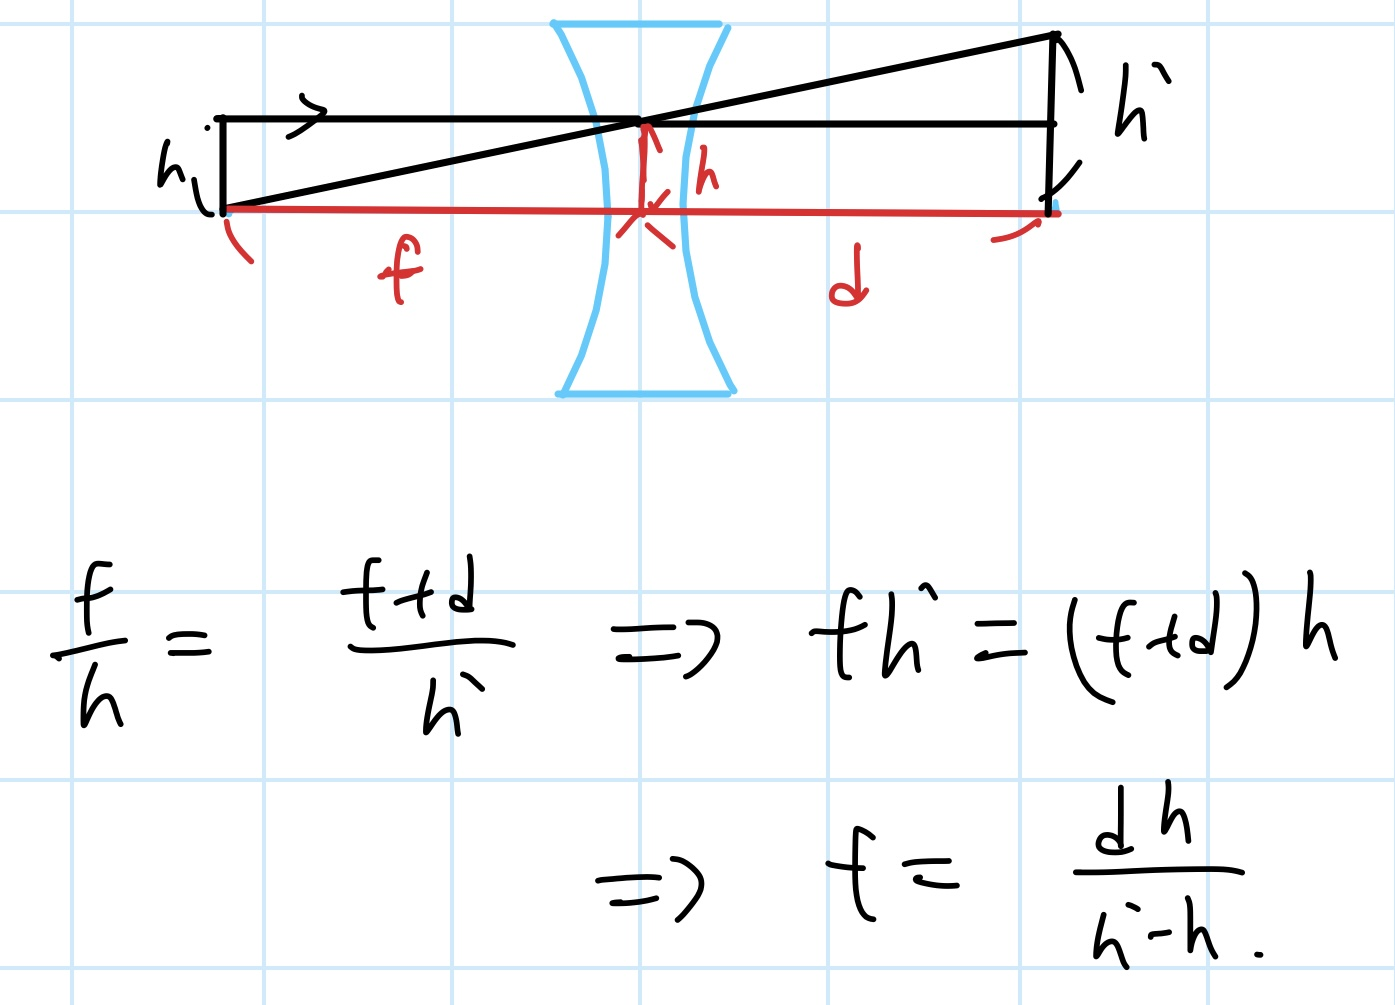
\includegraphics[width=120mm]{concave focal length.jpg}
    \caption{Diagram }
    \label{fig:concave_focal_diagram}
\end{figure}






\end{document}